\documentclass[11pt]{article}
\usepackage[T1]{fontenc}
\usepackage[utf8]{inputenc}
\usepackage[a4paper,margin=2.2cm]{geometry}
\usepackage{graphicx,booktabs,amsmath,url,hyperref,longtable}
\renewcommand{\thefigure}{S\arabic{figure}}
\renewcommand{\thetable}{S\arabic{table}}
\title{Supplementary material: Local Consumer Complaint Classification: Zero-Shot, Lightweight Adaptation and Label Budgets}
\author{Muhammet Tan and Halit Bak{\i}r}
\date{}
\begin{document}
\maketitle
Figure colours distinguish model groups; Fig.~\ref{fig:vs_reference}
marks Gemma's unspecified GGUF benchmark thinking mode separately.
Its placement in the standard colour group does not establish that
reasoning was disabled.
\section{Additional figures}
\begin{figure}[tb]
  \centering
  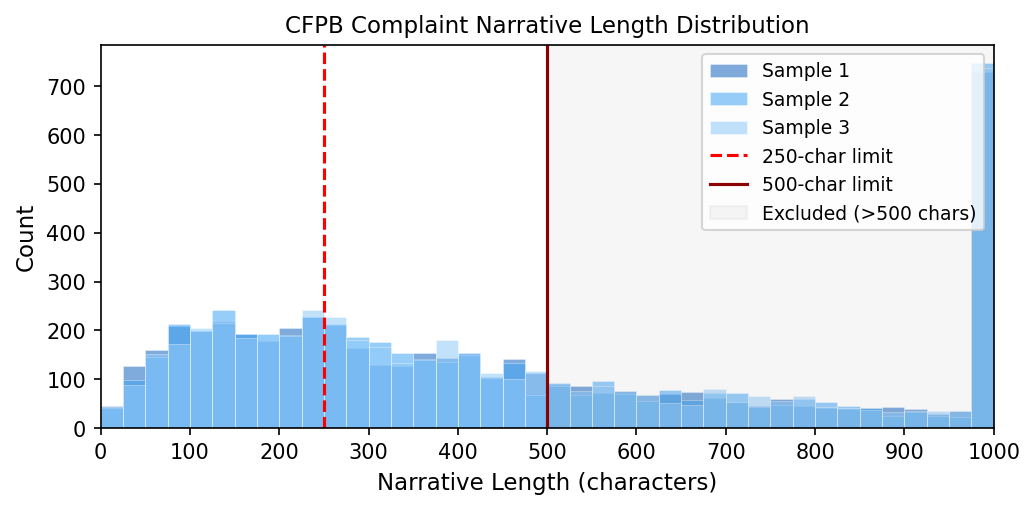
\includegraphics[width=\textwidth]{figures/v2/char_length_histogram.png}
  \caption{Narrative character-length distribution in three random
           $N{=}5{,}000$ samples from the unfiltered non-missing corpus
           (seeds 1--3, different colours), before test-set construction.
           Lengths at or above 1,000 characters are collected in the last bin.
           The dashed line marks the 250-character evaluation limit;
           the solid line marks 500 characters.
           The unfiltered corpus median is 361 characters; 42.7\,\%
           of narratives have at most 300 characters. These samples
           describe the source corpus rather than the balanced test sets.}
  \label{fig:char_hist}
\end{figure}\clearpage

\begin{figure}[tb]
  \centering
  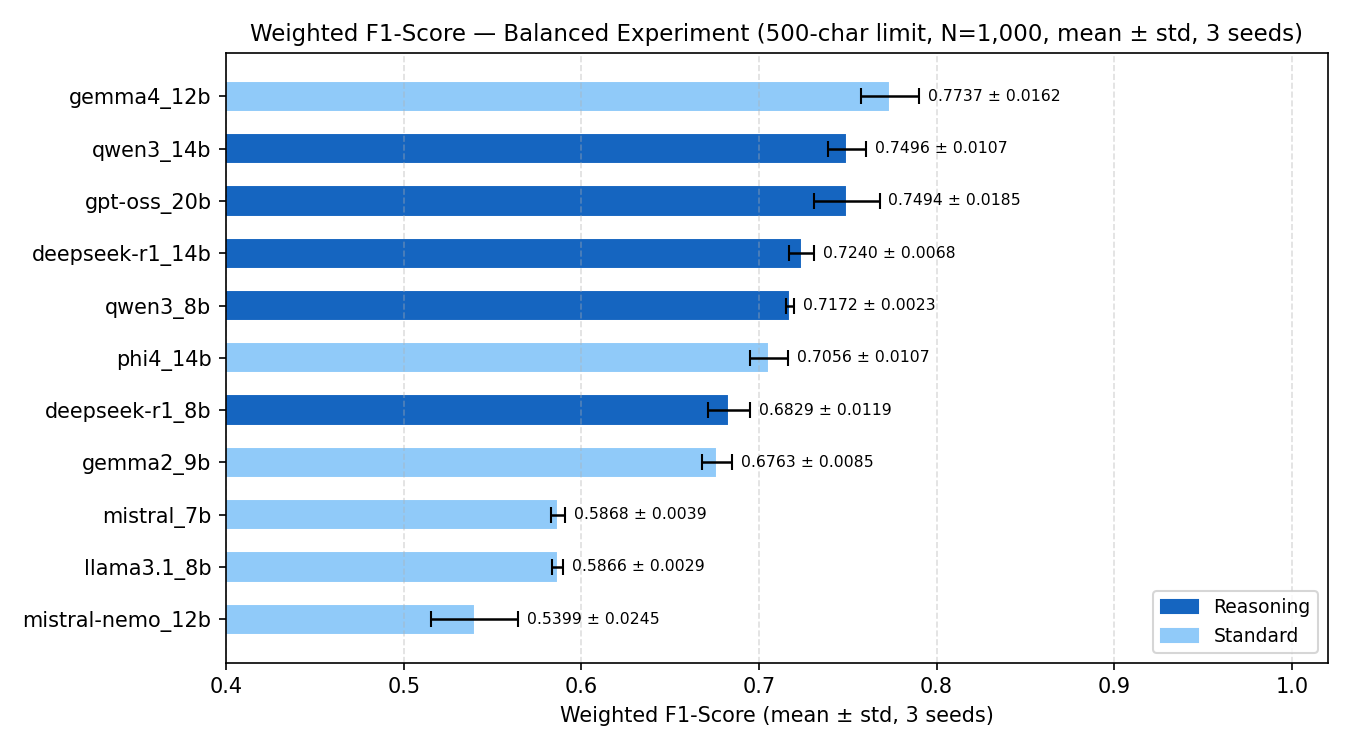
\includegraphics[width=\textwidth]{figures/v2/f1_balanced_errbar.png}
  \caption{Weighted F1-scores for all eleven models in Experiment~A (Balanced),
           shown as mean~$\pm$~sample std over three test subsets.
           Reasoning models are shown in dark blue; standard models in
           light blue under the original grouping. Gemma~4's thinking
           mode was not recorded; its original standard label is provisional.}
  \label{fig:f1_bar}
\end{figure}\clearpage

\begin{figure}[tb]
  \centering
  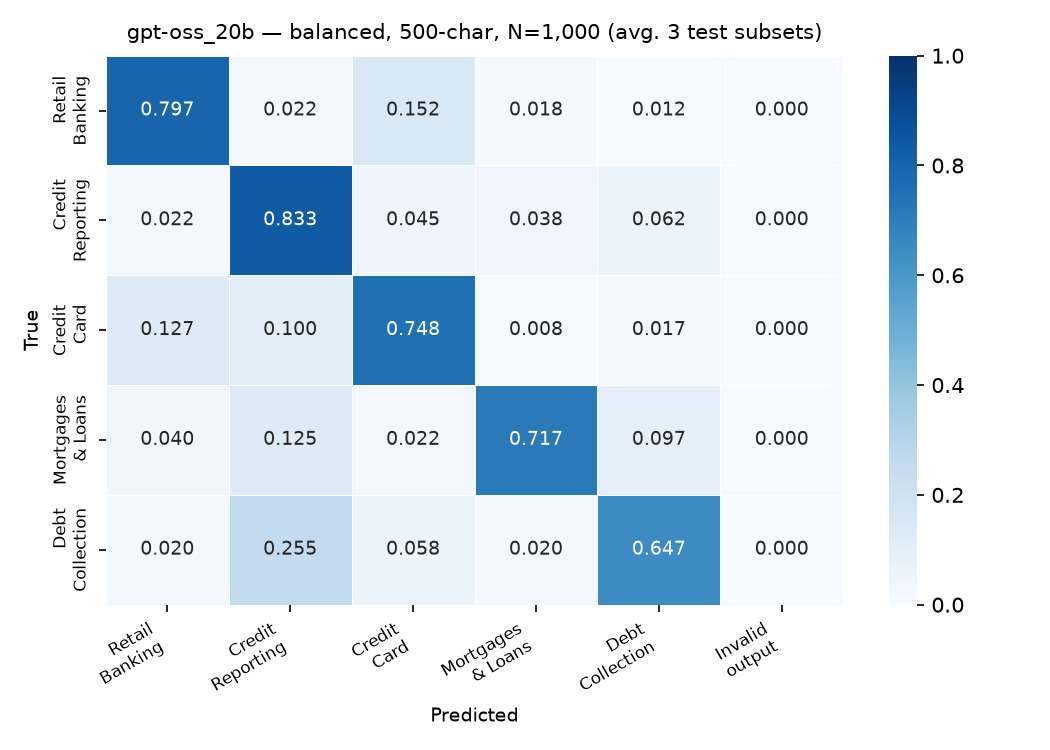
\includegraphics[width=0.92\textwidth]{figures/v2/confusion_gpt-oss_20b_balanced.png}
  \caption{Averaged confusion matrix for \texttt{gpt-oss:20b} (third-ranked
           model, Experiment~A, $N{=}1{,}000$, averaged
           over 3 test subsets). Cells are mean row-normalised proportions;
           rows are true labels and columns are predicted labels, with a
           separate invalid-output column.}
  \label{fig:conf_best}
\end{figure}\clearpage

\begin{figure}[tb]
  \centering
  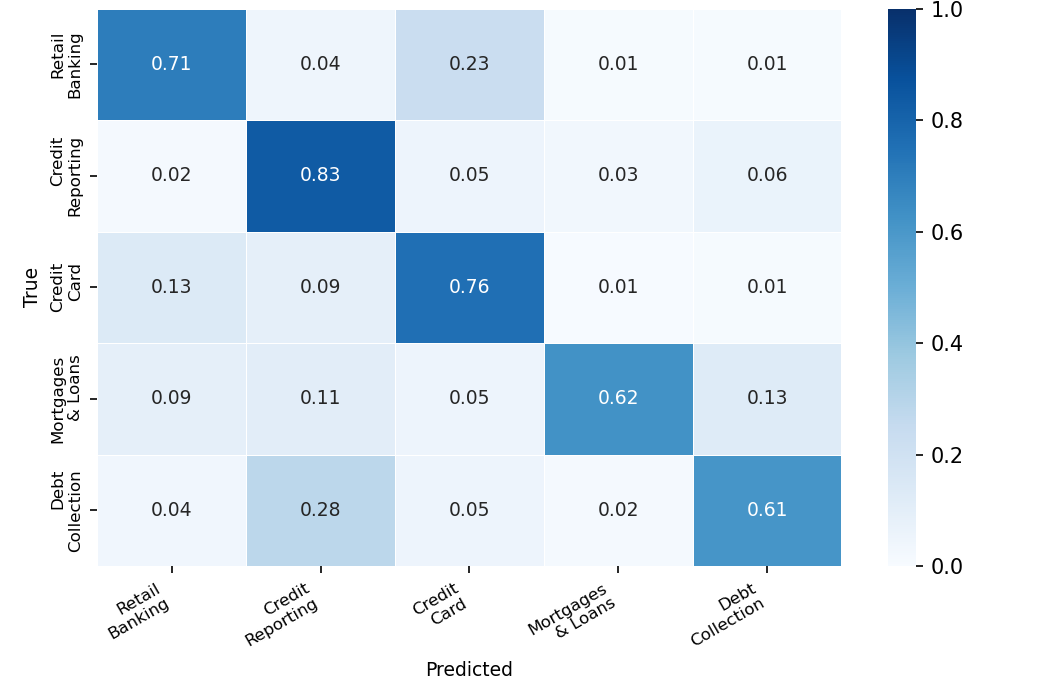
\includegraphics[width=0.92\textwidth]{figures/v2/confusion_phi4_14b_balanced.png}
  \caption{Averaged confusion matrix for \texttt{phi4:14b} (sixth overall,
           best sub-1-second standard model, Experiment~A, averaged over
           3 test subsets). Cells are mean row-normalised proportions;
           invalid outputs retain a separate error column. Prominent errors
           include debt collection predicted as credit reporting and retail
           banking predicted as credit card.}
  \label{fig:conf_phi4}
\end{figure}\clearpage

\begin{figure}[tb]
  \centering
  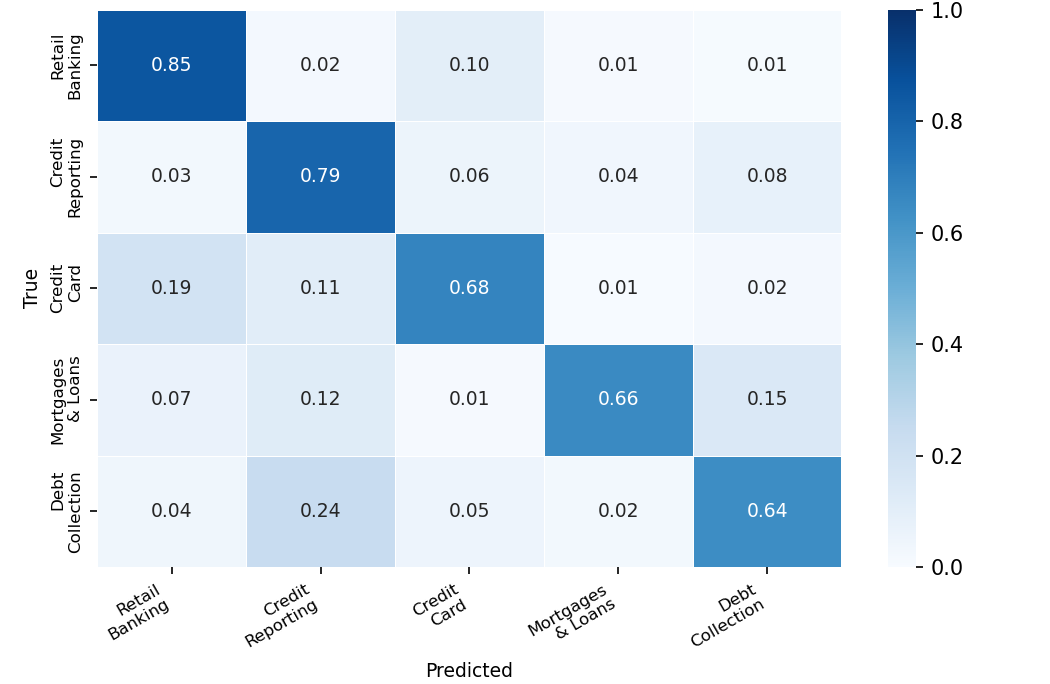
\includegraphics[width=0.92\textwidth]{figures/v2/confusion_deepseek-r1_14b_balanced.png}
  \caption{Averaged confusion matrix for \texttt{deepseek-r1:14b} (fourth-ranked
           model, third among the originally designated reasoning models, Experiment~A, averaged over
           3 test subsets). Cells are mean row-normalised proportions;
           invalid outputs retain a separate error column. Prominent errors
           include debt collection predicted as credit reporting and credit
           card predicted as retail banking.}
  \label{fig:conf_worst}
\end{figure}\clearpage

\begin{figure}[tb]
  \centering
  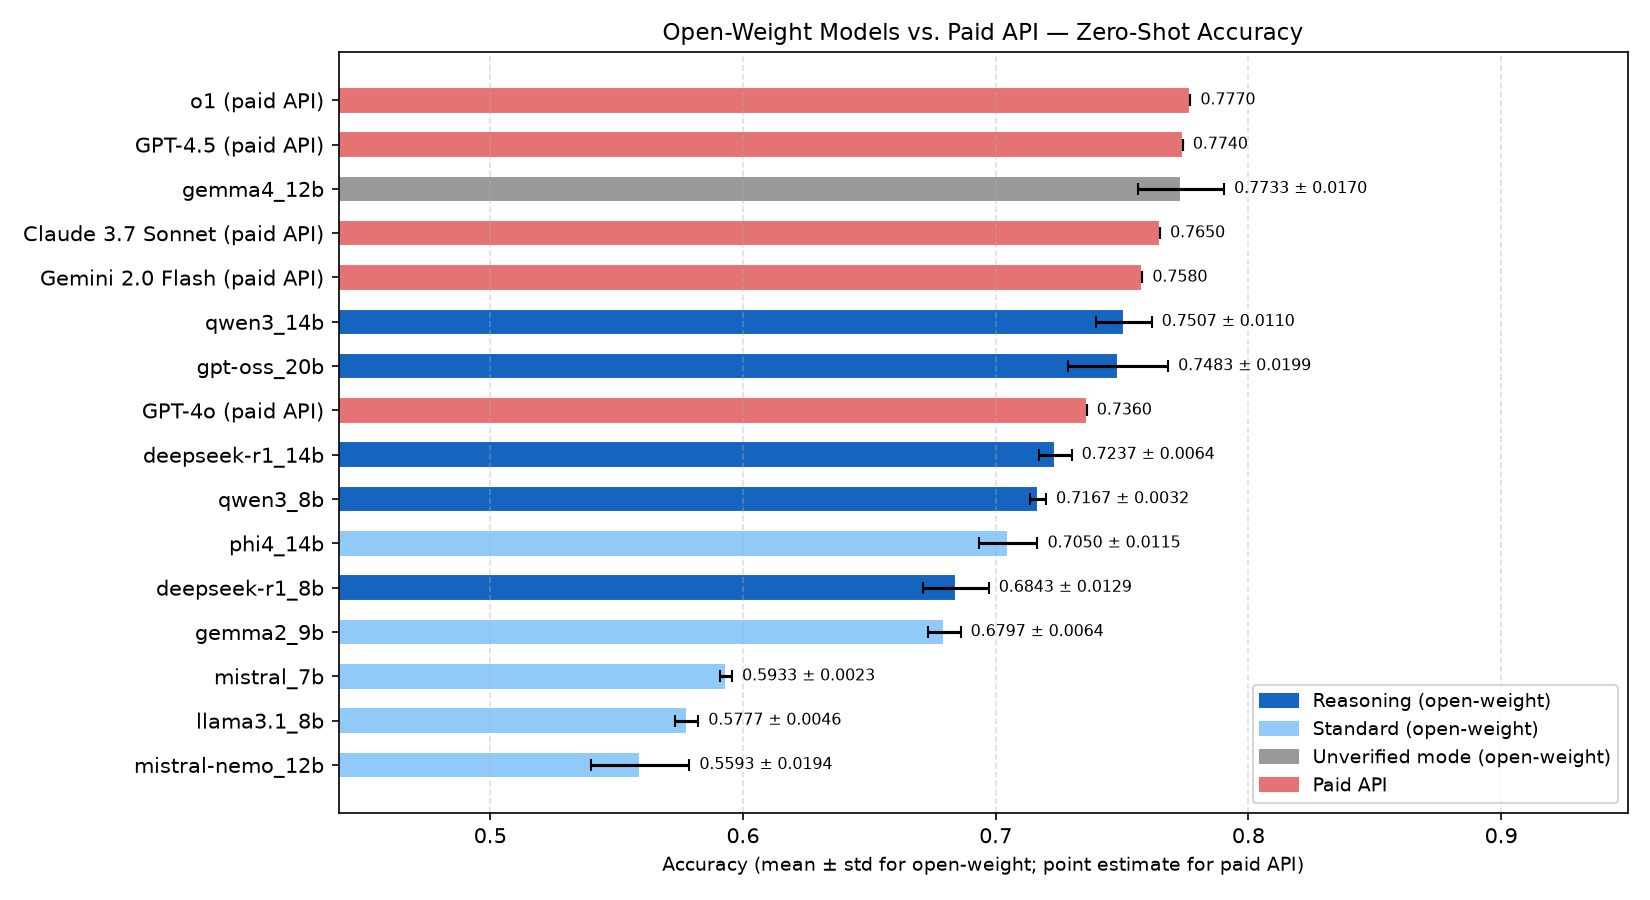
\includegraphics[width=\textwidth]{figures/v2/vs_reference.png}
  \caption{Accuracy of all eleven open-weight models (Experiment~A,
           mean~$\pm$~sample std over 3 test subsets) alongside five paid-API baselines
           from the literature \cite{roumeliotis2025think}.
           \texttt{gemma4:12b} is numerically close to GPT-4.5 and o1
           without API fees; this is not an equivalence test.
           Open-weight error bars reflect test-subset variability; paid-API
           figures are single-run point estimates.}
  \label{fig:vs_reference}
\end{figure}\clearpage

\begin{figure}[tb]
  \centering
  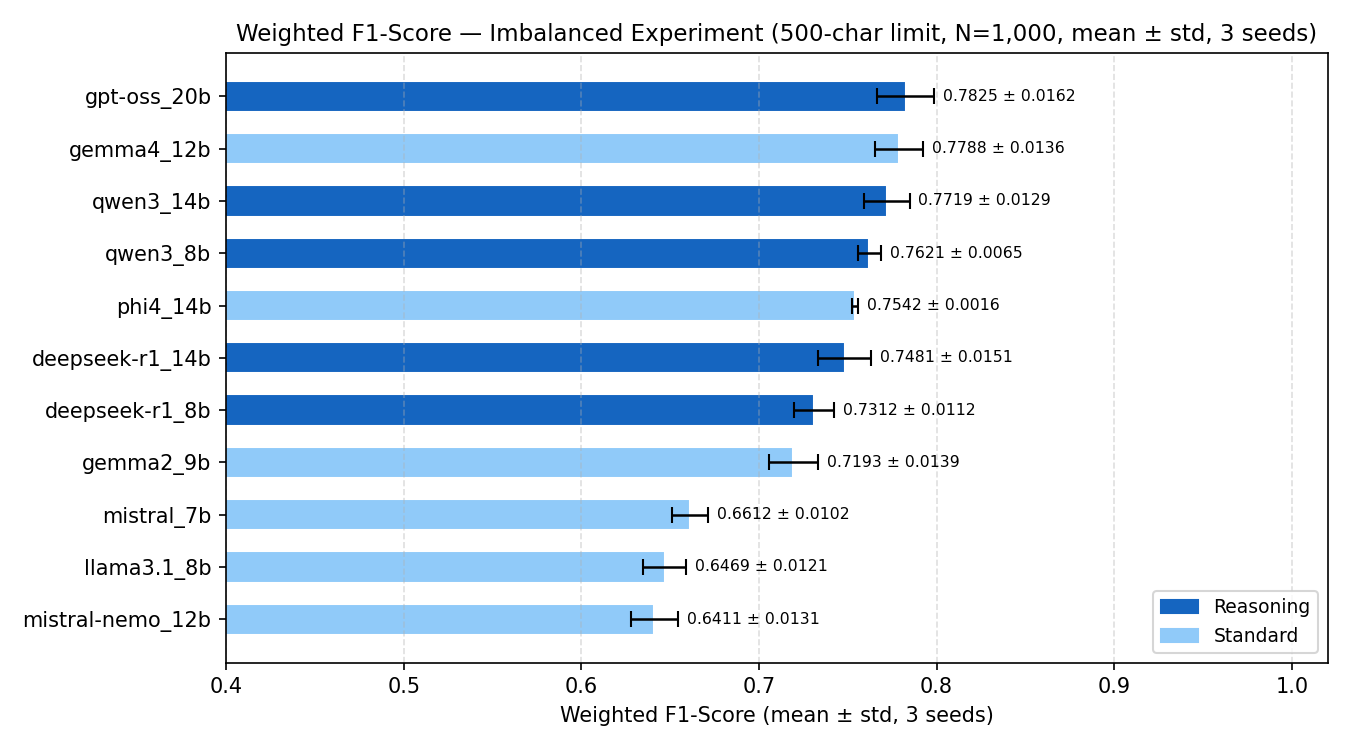
\includegraphics[width=\textwidth]{figures/v2/f1_imbalanced_errbar.png}
  \caption{Weighted F1-scores for all eleven models in Experiment~B
           (Imbalanced), shown as mean~$\pm$~sample std over three test subsets
           ($N{=}1{,}000$). Reasoning models are shown in dark blue;
           standard models in light blue. \texttt{gpt-oss:20b} leads,
           with \texttt{gemma4:12b} a close second.}
  \label{fig:f1_imbalanced}
\end{figure}\clearpage
\begin{figure}[tb]
  \centering
  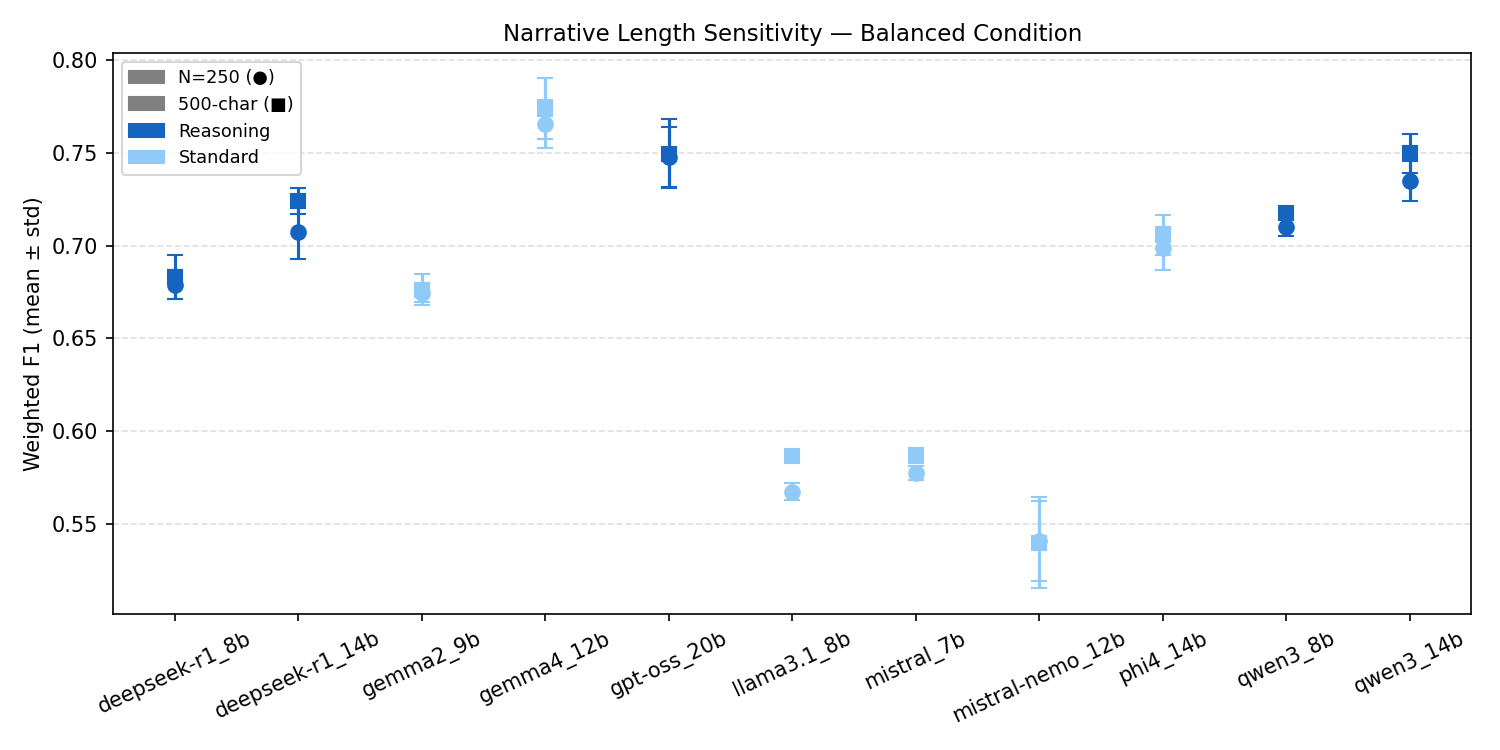
\includegraphics[width=\textwidth]{figures/v2/size_sensitivity_balanced.png}
  \caption{Mean accuracy on 250-char vs 500-char narrative variants
           (Balanced, $N{=}1{,}000$, 3 test subsets) for all eleven models.
           Rankings are highly stable; most models show small gains
           with longer narratives.}
  \label{fig:size_sensitivity}
\end{figure}\clearpage
\subsection{Within-Family Performance Patterns}

The eleven-model set permits several within-family comparisons.

\textbf{Gemma family (Google):} \texttt{gemma4:12b} (F1~0.774)
outperforms \texttt{gemma2:9b} (F1~0.676) by 0.098 F1 points —
the largest within-family gain observed. Off-label counts increase slightly from gemma2 (mean 0.3) to
gemma4 (mean 3.7); the latter are empty responses recorded as parse
errors. This comparison changes both generation (Gemma~2 to Gemma~4)
and parameter count (9B to 12B), and cannot separate their effects.

\textbf{Mistral family (Mistral AI):} \texttt{mistral-nemo:12b}
(F1~0.540) performs \emph{worse} than \texttt{mistral:7b} (F1~0.587)
in Experiment~A, despite having 71\,\% more parameters. Their
error modes are opposite: \texttt{mistral:7b} frequently produces
off-label outputs (58.7 per run), whereas \texttt{mistral-nemo:12b}
commits to valid categories but assigns them incorrectly.
Both mean latencies are below one second (0.23~s vs 0.59~s). This establishes a performance difference for the saved
configurations, but does not identify its architectural or training cause.

\textbf{Qwen3 family (Alibaba):} \texttt{qwen3:14b} (F1~0.750)
outperforms \texttt{qwen3:8b} (F1~0.717) consistently across both
experiments. Both have zero invalid outputs in balanced 500-character
tests; in Experiment~B, Qwen3~8B has one invalid output across the
three subsets and Qwen3~14B has none. The
+0.033 F1 gain is achieved with comparable latency (5.73~s vs 5.19~s),
alongside larger reported artifact size (9.3~GB vs 5.2~GB);
peak runtime VRAM was not recorded. Both models demonstrate that the Qwen3
configurations produce almost exclusively in-taxonomy outputs in these tests.

\textbf{DeepSeek-R1:} \texttt{deepseek-r1:14b}
(F1~0.724) outperforms \texttt{deepseek-r1:8b} (F1~0.683) by 0.041
F1 points. The 14B tag also has fewer invalid outputs (1.3 vs 2.0).
Latency increases (9.33~s vs 5.14~s); separate thinking traces
and token counts were not retained. The
performance gap is consistent across all three test subsets, but
the tags can also differ in backbone and model revision
\cite{guo2025deepseekr1,ollama2026deepseekregistry}. Missing artifact
digests prevent identifying a parameter-count effect from this pair.


\section{Saved splits and statistical units}
\label{sec:split_integrity}

Table~\ref{tab:split_inventory} summarises the saved data splits.
The benchmark is drawn from the length-filtered, deduplicated source
pool with master seed 42. Within each condition, consecutive class-wise
slices form subsets 1--3; seeds 42, 43 and 44 shuffle their row order.
The 250-character files shorten the same ordered records and are not
new samples. Across the two 500-character conditions, 2,067 normalised
texts are shared, leaving a union of 3,933 texts.

\begin{table}[htbp]\centering\small
\caption{Split inventory. Test counts are per saved 1,000-record subset;
each test condition has three subsets and two paired length variants.
RB/CR/CC/ML/DC denote retail banking, credit reporting, credit cards,
mortgages/loans and debt collection.}
\label{tab:split_inventory}
\begin{tabular}{lrl}\toprule
Split & Records & Class counts \\\midrule
Nested training & 500/2,000/10,000/20,000 & 100/400/2,000/4,000 per class \\
Fixed validation & 2,000 & 400 per class \\
Test A, each subset & 1,000 & 200 per class \\
Test B, each subset & 1,000 & RB 100, CR 511, CC 100, ML 107, DC 182 \\
\bottomrule\end{tabular}
\end{table}

Before supervised sampling, all twelve test files are reserved by
normalised-text hash and 250-character-prefix matching. Source candidates
with conflicting labels for one text hash are removed; MinHash/Jaccard
screening then excludes retrieved near matches to the tests.
Seed 42 draws the fixed balanced validation set and nested training
sets, with a further prefix/near-match exclusion against validation.
The saved source index traces a row of the processed CSV; it does not
identify a CFPB complaint, consumer or institution. These splits support
random-sample evaluation in this corpus, not temporal or source-group
generalisation. Training seeds 1--3 change optimisation randomness on
identical training and validation records.

The matched classifier comparison uses identical training/validation
records. Validation selects SVM's $C$ and DistilBERT's checkpoint by
weighted F1, while adapter checkpoints minimise completion-only loss.
SVM has one fixed-seed fit per budget; encoder and adapter summaries
describe three fits. Equal record counts control label availability,
not tuning effort, compute or the cost of obtaining individual labels.

A bootstrap cluster comprises all occurrences of the same normalised
input text within one condition and length, across its three test files.
Both modes receive the same cluster multiplicity in a resample. The
500-character conditions each contain 3,000 clusters; at 250 characters,
A contains 2,997 and B contains 2,986. None has conflicting cluster labels.
The paired implementation stratifies by true class when cluster labels
are consistent and otherwise uses unstratified cluster resampling.
McNemar uses one occurrence per source-input hash, keeping the first
subset/index; conflicting-label source inputs would be excluded from
that accuracy test, rather than from the F1 denominator. The 133 excluded
source-corpus conflicting-label groups concern supervised split
construction. Holm correction does not require independent comparisons,
but cannot make overlapping tests independent replications.

For the equal-prior diagnostic, let $C_{ij}$ be the pooled confusion
matrix, including an invalid-output column, and $n_i=\sum_j C_{ij}$.
We compute $\widetilde C_{ij}=C_{ij}/n_i$, retaining fractional counts,
then recompute precision, recall and F1 from $\widetilde C$.
No rounding is applied before metric calculation. Each row has unit
support, so macro and weighted F1 coincide under this diagnostic prior;
this changes the weighting of observed errors, not the predictions.

\section{Controlled HF adaptation: complete results and reproducibility}
Three models use the same 500 balanced training and 2,000 validation records,
with three training seeds each. Nine base/adapted pairs use identical
pinned weights within each fit. Exact revisions are:
% Generated by export_qlora_manuscript.py from verified saved predictions.

\begin{description}
\item[Gemma 4] \path{google/gemma-4-12B-it}, revision \path{707f0a3b8a3c7ad586ed01e27eafbad8a27dd0f7}.
\item[Qwen3] \path{Qwen/Qwen3-14B}, revision \path{40c069824f4251a91eefaf281ebe4c544efd3e18}.
\item[Phi-4] \path{microsoft/phi-4}, revision \path{2db69c1c3e91a05d2c64a3185acfbaf36f744e25}.
\end{description}

All 216,000 test predictions and 1,800 serial predictions pass the same
source, label, hash, response and pairing checks. Mean and sample standard
deviation describe three fits on the same tests, not 9,000 independent
records. Per-fit paired confidence intervals and unique-input McNemar tests
use the original cluster and duplicate handling. Holm correction covers
36 base/adapter comparisons; a separate family of 72 tests compares
adapters with label-matched SVM and validation-stopped DistilBERT.
Serial timing uses the same first 20 records per class from the first
balanced 500-character file; full-test scores use batched predictions.
For the eleven-model GGUF script, request timing stops when the HTTP
response headers arrive, before reading and parsing the response body.
Each saved row records the final attempt; retry waits and preceding
attempts are excluded. Invalid/error rows remain in the reported means.
This boundary differs from the thinking control's complete HTTP timing
and the HF generation benchmark; the timings are not interchangeable.

The initial seed-1 results are retained for traceability in
Table~\ref{tab:qlora_full} (full metrics), Table~\ref{tab:qlora_class}
(class metrics), and Table~\ref{tab:qlora_serial} (timing and agreement).
These three tables describe seed 1, not averages over fits.
% Generated by export_qlora_manuscript.py from verified saved predictions.
\begin{table}[tb]
\centering
\footnotesize
\setlength{\tabcolsep}{3pt}
\caption{Seed-1 HF paired comparison (seed-1 twelve-test correction family). A: balanced; B: reduced imbalance; chars: narrative limit. Each row pools 3,000 records per mode. F1w/F1m: weighted/macro F1. Gain and CI are percentage points; $p_H$ is the exact accuracy McNemar p-value after Holm correction over twelve comparisons.}
\label{tab:qlora_full}
\begin{tabular}{llrrrrrrr}
\toprule
Model & Cond. & Chars & Base F1w & QLoRA F1w & QLoRA F1m & $\Delta$ & 95\,\% CI & $p_H$ \\
\midrule
Gemma 4 & A & 250 & 0.7461 & 0.7674 & 0.7674 & +2.13 & [1.03, 3.24] & 0.00019 \\
Gemma 4 & A & 500 & 0.7520 & 0.7803 & 0.7803 & +2.83 & [1.75, 3.96] & 1.3e-06 \\
Gemma 4 & B & 250 & 0.7689 & 0.7862 & 0.7472 & +1.73 & [0.64, 2.81] & 0.0014 \\
Gemma 4 & B & 500 & 0.7730 & 0.7948 & 0.7576 & +2.18 & [1.12, 3.22] & 0.00015 \\
Qwen3 & A & 250 & 0.7050 & 0.7767 & 0.7767 & +7.17 & [5.80, 8.55] & 7.9e-20 \\
Qwen3 & A & 500 & 0.7099 & 0.7891 & 0.7891 & +7.92 & [6.55, 9.34] & 8.1e-23 \\
Qwen3 & B & 250 & 0.7210 & 0.7826 & 0.7453 & +6.16 & [4.81, 7.49] & 3.6e-17 \\
Qwen3 & B & 500 & 0.7278 & 0.7946 & 0.7602 & +6.68 & [5.30, 8.07] & 7.8e-18 \\
Phi-4 & A & 250 & 0.6824 & 0.7794 & 0.7794 & +9.70 & [8.24, 11.16] & 6.3e-37 \\
Phi-4 & A & 500 & 0.6883 & 0.7845 & 0.7845 & +9.62 & [8.21, 11.07] & 7.5e-36 \\
Phi-4 & B & 250 & 0.7406 & 0.7947 & 0.7598 & +5.41 & [4.08, 6.72] & 6.4e-15 \\
Phi-4 & B & 500 & 0.7456 & 0.7994 & 0.7643 & +5.38 & [4.08, 6.68] & 2.6e-14 \\
\bottomrule
\end{tabular}
\end{table}
\begin{table}[tb]
\centering
\footnotesize
\setlength{\tabcolsep}{3pt}
\caption{Seed-1 pooled per-class F1 on 500-character tests. A/B denote balanced/reduced imbalance. Mortg.: mortgages and loans.}
\label{tab:qlora_class}
\begin{tabular}{lllrrrrr}
\toprule
Model & Cond. & Mode & Retail & Credit rep. & Card & Mortg. & Debt \\
\midrule
Gemma 4 & A & base & 0.8029 & 0.7120 & 0.7376 & 0.7996 & 0.7077 \\
Gemma 4 & A & adapter & 0.8410 & 0.7376 & 0.7552 & 0.8257 & 0.7418 \\
Gemma 4 & B & base & 0.7417 & 0.8427 & 0.6699 & 0.7315 & 0.6756 \\
Gemma 4 & B & adapter & 0.7927 & 0.8601 & 0.6645 & 0.7745 & 0.6960 \\
Qwen3 & A & base & 0.7423 & 0.6941 & 0.6970 & 0.8007 & 0.6154 \\
Qwen3 & A & adapter & 0.8318 & 0.7392 & 0.7739 & 0.8182 & 0.7822 \\
Qwen3 & B & base & 0.6463 & 0.8216 & 0.6042 & 0.7049 & 0.5906 \\
Qwen3 & B & adapter & 0.7748 & 0.8501 & 0.6728 & 0.7744 & 0.7287 \\
Phi-4 & A & base & 0.6820 & 0.6998 & 0.6761 & 0.7209 & 0.6628 \\
Phi-4 & A & adapter & 0.8302 & 0.7370 & 0.7429 & 0.8291 & 0.7832 \\
Phi-4 & B & base & 0.6371 & 0.8472 & 0.5891 & 0.6876 & 0.6402 \\
Phi-4 & B & adapter & 0.7963 & 0.8569 & 0.6656 & 0.7754 & 0.7273 \\
\bottomrule
\end{tabular}
\end{table}
\begin{table}[tb]
\centering
\footnotesize
\setlength{\tabcolsep}{3pt}
\caption{Seed-1 warm serial latency distribution on 100 fixed class-balanced records per model/mode. Agreement is with the corresponding saved full-test batched labels; full-test F1 is not replaced by the 100-record benchmark score.}
\label{tab:qlora_serial}
\begin{tabular}{llrrrr}
\toprule
Model & Mode & Mean (s) & Median (s) & P95 (s) & Agreement (\%) \\
\midrule
Gemma 4 & base & 0.475 & 0.470 & 0.577 & 100 \\
Gemma 4 & adapter & 0.647 & 0.627 & 0.791 & 99 \\
Qwen3 & base & 0.421 & 0.416 & 0.487 & 98 \\
Qwen3 & adapter & 0.539 & 0.540 & 0.627 & 100 \\
Phi-4 & base & 0.487 & 0.488 & 0.560 & 100 \\
Phi-4 & adapter & 0.435 & 0.429 & 0.510 & 100 \\
\bottomrule
\end{tabular}
\end{table}

Table~\ref{tab:replication_full} reports all three training seeds.
\begingroup\scriptsize
\begin{longtable}{llrrrrrr}
\caption{Complete three-training-seed paired results, each pooled over
the same 3,000 test records. A/B denote balanced/reduced imbalance;
the length column is a character limit, not a sample size.
Holm $p$ tests accuracy differences across the full 36-comparison family;
it does not test the displayed F1 difference. Gain intervals are unadjusted
95\,\% paired cluster-bootstrap intervals in percentage points.}
\label{tab:replication_full}\\
\toprule Model & Test & Length & Fit seed & Base F1 & Adapted F1 & Gain [95\,\% CI] (pp) & Holm $p$ \\\midrule
\endfirsthead
\toprule Model & Test & Length & Fit seed & Base F1 & Adapted F1 & Gain [95\,\% CI] (pp) & Holm $p$ \\\midrule
\endhead
Gemma 4 & A & 250 & 1 & 0.7461 & 0.7674 & 2.13 [1.03, 3.24] & 0.000575 \\
Gemma 4 & A & 250 & 2 & 0.7461 & 0.7868 & 4.07 [2.89, 5.23] & 3.55e-11 \\
Gemma 4 & A & 250 & 3 & 0.7461 & 0.7703 & 2.42 [1.34, 3.48] & 0.000139 \\
Gemma 4 & A & 500 & 1 & 0.7520 & 0.7803 & 2.83 [1.75, 3.96] & 3.85e-06 \\
Gemma 4 & A & 500 & 2 & 0.7520 & 0.7952 & 4.33 [3.16, 5.55] & 4.32e-12 \\
Gemma 4 & A & 500 & 3 & 0.7520 & 0.7768 & 2.48 [1.40, 3.55] & 0.000104 \\
Gemma 4 & B & 250 & 1 & 0.7689 & 0.7862 & 1.73 [0.64, 2.81] & 0.00566 \\
Gemma 4 & B & 250 & 2 & 0.7689 & 0.7751 & 0.62 [-0.51, 1.76] & 1 \\
Gemma 4 & B & 250 & 3 & 0.7689 & 0.7868 & 1.78 [0.73, 2.84] & 0.00574 \\
Gemma 4 & B & 500 & 1 & 0.7730 & 0.7948 & 2.18 [1.12, 3.22] & 0.000345 \\
Gemma 4 & B & 500 & 2 & 0.7730 & 0.7814 & 0.84 [-0.31, 2.02] & 1 \\
Gemma 4 & B & 500 & 3 & 0.7730 & 0.7944 & 2.15 [1.08, 3.19] & 0.000968 \\
Phi-4 & A & 250 & 1 & 0.6824 & 0.7794 & 9.70 [8.24, 11.16] & 1.85e-36 \\
Phi-4 & A & 250 & 2 & 0.6821 & 0.7769 & 9.48 [7.99, 10.95] & 5.14e-34 \\
Phi-4 & A & 250 & 3 & 0.6821 & 0.7750 & 9.29 [7.87, 10.71] & 7.99e-35 \\
Phi-4 & A & 500 & 1 & 0.6883 & 0.7845 & 9.62 [8.21, 11.07] & 2.32e-35 \\
Phi-4 & A & 500 & 2 & 0.6886 & 0.7859 & 9.72 [8.29, 11.22] & 8.81e-35 \\
Phi-4 & A & 500 & 3 & 0.6886 & 0.7867 & 9.81 [8.42, 11.18] & 5.96e-39 \\
Phi-4 & B & 250 & 1 & 0.7406 & 0.7947 & 5.41 [4.08, 6.72] & 1.91e-14 \\
Phi-4 & B & 250 & 2 & 0.7404 & 0.7749 & 3.45 [2.11, 4.81] & 9.07e-05 \\
Phi-4 & B & 250 & 3 & 0.7404 & 0.7824 & 4.20 [2.90, 5.46] & 7.15e-08 \\
Phi-4 & B & 500 & 1 & 0.7456 & 0.7994 & 5.38 [4.08, 6.68] & 8.98e-14 \\
Phi-4 & B & 500 & 2 & 0.7464 & 0.7857 & 3.94 [2.62, 5.27] & 6.09e-06 \\
Phi-4 & B & 500 & 3 & 0.7464 & 0.7899 & 4.35 [3.06, 5.66] & 4.24e-08 \\
Qwen3 & A & 250 & 1 & 0.7050 & 0.7767 & 7.17 [5.80, 8.55] & 2.36e-19 \\
Qwen3 & A & 250 & 2 & 0.7050 & 0.7695 & 6.45 [5.14, 7.82] & 2.52e-17 \\
Qwen3 & A & 250 & 3 & 0.7050 & 0.7771 & 7.21 [5.84, 8.62] & 1.83e-20 \\
Qwen3 & A & 500 & 1 & 0.7099 & 0.7891 & 7.92 [6.55, 9.34] & 2.34e-22 \\
Qwen3 & A & 500 & 2 & 0.7099 & 0.7727 & 6.28 [4.95, 7.61] & 5.26e-16 \\
Qwen3 & A & 500 & 3 & 0.7099 & 0.7880 & 7.81 [6.46, 9.18] & 1.17e-23 \\
Qwen3 & B & 250 & 1 & 0.7210 & 0.7826 & 6.16 [4.81, 7.49] & 1.12e-16 \\
Qwen3 & B & 250 & 2 & 0.7210 & 0.7767 & 5.56 [4.24, 6.87] & 1.11e-14 \\
Qwen3 & B & 250 & 3 & 0.7210 & 0.7831 & 6.20 [4.85, 7.56] & 3.34e-17 \\
Qwen3 & B & 500 & 1 & 0.7278 & 0.7946 & 6.68 [5.30, 8.07] & 2.52e-17 \\
Qwen3 & B & 500 & 2 & 0.7278 & 0.7852 & 5.74 [4.47, 7.07] & 1.11e-14 \\
Qwen3 & B & 500 & 3 & 0.7278 & 0.7931 & 6.53 [5.13, 7.89] & 3.1e-17 \\
\bottomrule\end{longtable}

\endgroup
Table~\ref{tab:replication_class} reports class F1 averaged over all
three training fits, complementing the seed-1 audit table.
% Generated from verified qlora_per_fit.csv, three independent adapter fits.
\begin{table}[tb]
\centering\scriptsize
\setlength{\tabcolsep}{3pt}
\caption{Adapted class F1 on 500-character tests, mean $\pm$ sample
standard deviation over three training fits, each evaluated on the same
3,000 records per condition. A/B denote balanced/reduced imbalance;
Mortg. denotes mortgages and loans.}
\label{tab:replication_class}
\begin{tabular}{llrrrrr}\toprule
Model & Test & Retail & Credit rep. & Card & Mortg. & Debt \\\midrule
Gemma 4 & A & $0.8398\pm0.0013$ & $0.7408\pm0.0111$ & $0.7631\pm0.0073$ & $0.8218\pm0.0155$ & $0.7550\pm0.0215$ \\
Qwen3 & A & $0.8308\pm0.0016$ & $0.7392\pm0.0120$ & $0.7626\pm0.0137$ & $0.8124\pm0.0079$ & $0.7714\pm0.0133$ \\
Phi-4 & A & $0.8327\pm0.0031$ & $0.7399\pm0.0026$ & $0.7434\pm0.0039$ & $0.8336\pm0.0045$ & $0.7789\pm0.0046$ \\
Gemma 4 & B & $0.7900\pm0.0027$ & $0.8511\pm0.0148$ & $0.6660\pm0.0024$ & $0.7625\pm0.0153$ & $0.7040\pm0.0106$ \\
Qwen3 & B & $0.7830\pm0.0071$ & $0.8496\pm0.0017$ & $0.6650\pm0.0119$ & $0.7622\pm0.0126$ & $0.7169\pm0.0130$ \\
Phi-4 & B & $0.7969\pm0.0028$ & $0.8481\pm0.0080$ & $0.6398\pm0.0246$ & $0.7796\pm0.0040$ & $0.7208\pm0.0070$ \\
\bottomrule\end{tabular}\end{table}

\subsection{Completion length and warm serial timing}
\label{sec:serial_tokens}
Table~\ref{tab:serial_tokens} reports the same 100 balanced records
per mode and fit (20 per class), including end-of-turn tokens.
All recorded output-limit counts are zero. These are serial benchmark
outputs; their token counts are not substituted for full-test metrics.
Adapter execution and response length both change between modes,
so this table describes their joint observation rather than isolating
either contribution to latency.
\begin{table}[tb]\centering\small
\caption{Per-fit serial completion length and latency. Token counts and
latency are means over 100 requests in each mode; seconds include prompt
rendering, tokenisation and synchronised generation.}
\label{tab:serial_tokens}
\begin{tabular}{llrrrr}\toprule
Model & Fit seed & Base tokens & Adapted tokens & Base (s) & Adapted (s) \\\midrule
Gemma 4 & 1 & 9.48 & 9.57 & 0.475 & 0.647 \\
Gemma 4 & 2 & 9.48 & 9.60 & 0.482 & 0.659 \\
Gemma 4 & 3 & 9.48 & 9.54 & 0.490 & 0.661 \\
Qwen3 & 1 & 9.27 & 9.35 & 0.421 & 0.539 \\
Qwen3 & 2 & 9.27 & 9.30 & 0.422 & 0.539 \\
Qwen3 & 3 & 9.27 & 9.34 & 0.421 & 0.539 \\
Phi-4 & 1 & 13.01 & 9.36 & 0.487 & 0.435 \\
Phi-4 & 2 & 13.01 & 9.35 & 0.487 & 0.435 \\
Phi-4 & 3 & 13.01 & 9.32 & 0.490 & 0.440 \\
\bottomrule\end{tabular}\end{table}

\subsection{Thinking-control protocol and class metrics}
\label{sec:thinking_protocol}
The evaluation uses selection seed 20261009, a total generation cap of 4096 tokens
in both modes and both models, an 8,192-token context, temperature zero
and Ollama 0.35.0. No JSON grammar is forced.
The ten balanced pilot records are excluded from the 500 evaluation
records by normalised-text hash. Selection precedes all pilot outputs;
the cap is selected from termination/empty-final flags, never accuracy.
Each request stores its full prompt/options, separate reasoning and final
response, token counts, termination reason, loading/generation duration
and serial HTTP wall time. Cluster-stratified paired bootstrap uses
5,000 draws; two exact two-sided McNemar tests use Holm correction.
Raw outputs and manifests are in
\path{results/sadhana/thinking_control_20261009/}.
At the highest prespecified cap, one excluded Gemma thinking-on
pilot input still terminates at the length limit. A technical
amendment recorded before any main predictions fixes this finite
budget instead of extending the search. All length-terminated main
responses count as errors, including any embedded JSON; the two modes
retain identical budgets and unchanged input selection.
\begin{itemize}
\item gemma4:12b (Q4\_K\_M): artifact digest \newline\texttt{6114515d63c17436a7c0417d82820ac65ad643e2806c5a3c89cb62846436ed0b}.
\item qwen3:14b (Q4\_K\_M): artifact digest \newline\texttt{bdbd181c33f2ed1b31c972991882db3cf4d192569092138a7d29e973cd9debe8}.
\end{itemize}
Table~\ref{tab:thinking_class} reports per-class F1.
\begin{table}[tb]\centering\small
\caption{Class F1 in the controlled thinking experiment.}
\label{tab:thinking_class}
\begin{tabular}{llrrrrr}\toprule
Model & Mode & Retail & CreditRep. & Card & Mortg. & Debt \\\midrule
Gemma 4 & Off & 0.7729 & 0.7059 & 0.7400 & 0.7527 & 0.6774 \\
Gemma 4 & On & 0.8131 & 0.7407 & 0.7363 & 0.7312 & 0.7021 \\
Qwen3 & Off & 0.7206 & 0.6606 & 0.6811 & 0.7459 & 0.6545 \\
Qwen3 & On & 0.7879 & 0.7249 & 0.7333 & 0.7500 & 0.7283 \\
\bottomrule\end{tabular}\end{table}

Full seed summaries, class scores, baseline differences, bootstrap
intervals, adjusted tests and verification logs are supplied as CSV/JSON
reproducibility artifacts in the replication directory.
\clearpage

\section{Extended related work}
Complaint analysis spans several tasks that should be distinguished when
comparing results. Vasudeva~Raju~et~al.\ \cite{raju2022bertopic} evaluate
BERTopic and domain-specific FinBERT embeddings for topic discovery;
this is not a directly comparable five-label classification benchmark.
Vairetti~et~al.\ \cite{vairetti2024bert} address complaint prioritisation
using deep learning and multicriteria decision-making, while Das~et~al.\
\cite{das2024explainable} focus on interpretability in financial complaints.
Yuan~et~al.\ \cite{liu2024framework} examine LLM-based categorisation,
and Correa~et~al.\ \cite{correa2024genai} study classification,
summarisation and response generation for consumer communications.
These task differences preclude treating published accuracy values as
instance-matched targets for our preserved test sets.

The closest reference is Roumeliotis~et~al.\ \cite{roumeliotis2025think},
whose balanced 1,000-record, five-category CFPB evaluation reports
accuracy 0.777 and weighted F1 0.7764 for o1. Their exact sampled
identifiers are unavailable, so the commercial comparison remains
at the protocol level. Other tourism, e-commerce and customer-service
studies \cite{roumeliotis2024tourism,roumeliotis2024ecommerce,
li2024customerservice} provide context on generative-model deployment
rather than comparable scores on this dataset.

Shin~et~al.\ \cite{shin2025llmwritten} examine LLM adoption and efficacy
through financial-industry complaints. Liang~et~al.\ \cite{liang2025cfpb}
study LLM-assisted writing across several domains. Their work motivates
future evaluation on more recent complaint corpora; our processed data
and experiment design do not establish robustness to this shift.

Bulgakov and Turchin \cite{bulgakov2026deepseek} combine reasoning-based
predictions with a supervised correction stage for rare events in medical
and consumer-service data. G{\"u}ll{\"u}~et~al.\ \cite{gullu2025llama}
study customer complaint classification with LLMs. We do not import
numerical performance claims from these studies as direct comparators.
The present study evaluates the deployment choices supported by our
own zero-shot predictions, paired adaptation outputs and supervised
learning curve.

\bibliographystyle{unsrturl}
\bibliography{references}
\end{document}
